\documentclass[10pt, compress]{beamer}

\usetheme{m}
\usepackage{soul}

\usepackage{natbib}
\bibliographystyle{unsrt}
\usepackage{booktabs}
\usepackage[scale=2]{ccicons}
\usepackage{minted}
\usepackage{wrapfig}
\usepackage{enumitem}
\usemintedstyle{trac}
\usepackage{float}

\newcolumntype{C}[1]{>{\centering\let\newline\\\arraybackslash\hspace{0pt}}m{#1}}

\setbeameroption{show notes}

\begin{document}

\begin{frame}[plain,t]

\begin{wrapfigure}{r}{0.2\textwidth}
\begin{flushright}
\vspace{-2cm}

\includegraphics[width = 10mm]{figures/kth_logo.png}
\end{flushright}
\end{wrapfigure}

\vspace{2cm}

{\large\textbf{Planar graphs with girth at least 5 are (3,4)-colorable}}
\\\rule{10.25cm}{1pt}

\vspace{0.5cm}

{\large Presented by: \textbf{Phillip Gajland}}

\begin{figure}
\centering
\begin{subfigure}{.3\textwidth}
\centering

\includegraphics[width=.3\linewidth]{figures/logo1.png}
\end{subfigure}%
\begin{subfigure}{.3\textwidth}
\centering

\includegraphics[width=.3\linewidth]{figures/logo2.png}
\end{subfigure}%
\begin{subfigure}{.3\textwidth}
\centering

\includegraphics[width=.3\linewidth]{figures/logo3.jpg}
\end{subfigure}
\end{figure}

\begin{table}[]
\centering
\begin{tabular}{C{3cm} C{3cm} C{3cm}}
Ilkyoo Choi & Gexin Yu & Xia Zhang
\end{tabular}
\end{table}
% \vspace{0.5cm}
% {Published in: Discrete Mathematics, Volume 342, Issue 12, 2019}
\end{frame}

\begin{frame}{The Paper}
\vspace{1cm}
\begin{center}
\centering
{\LARGE\textbf{"Planar graphs with girth at least 5 are (3,4)-colorable"}}
\end{center}
\end{frame}

\begin{frame}{The Authors}
\begin{center}
\begin{table}[]
\centering
\begin{tabular}{l l}
Ilkyoo Choi & Hankuk University of Foreign Studies (HUFS)\\
Gexin Yu & The College of William and Mary\\
Xia Zhang & Shangdong Normal University
\end{tabular}
\end{table}
\begin{figure}[!tbp]
\centering
\begin{minipage}[b]{0.2\textwidth}

\includegraphics[width=\textwidth,height=2.25cm]{figures/choi.png}
\end{minipage}
\hfill
\begin{minipage}[b]{0.2\textwidth}
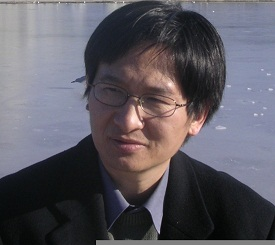
\includegraphics[width=\textwidth,height=2.25cm]{figures/yu.jpg}
\end{minipage}
\hfill
\begin{minipage}[b]{0.2\textwidth}

\includegraphics[width=\textwidth,height=2.25cm]{figures/zhang.png}
\end{minipage}
\end{figure}
\end{center}
\end{frame}

\begin{frame}{The Journal}
\begin{table}
\centering
\begin{tabular}{l l}
Name: & Discrete Mathematics\\
Volume: & 342, Issue 12\\
Date: & December 2019
\end{tabular}
\end{table}
\begin{figure}[!tbp]
\centering
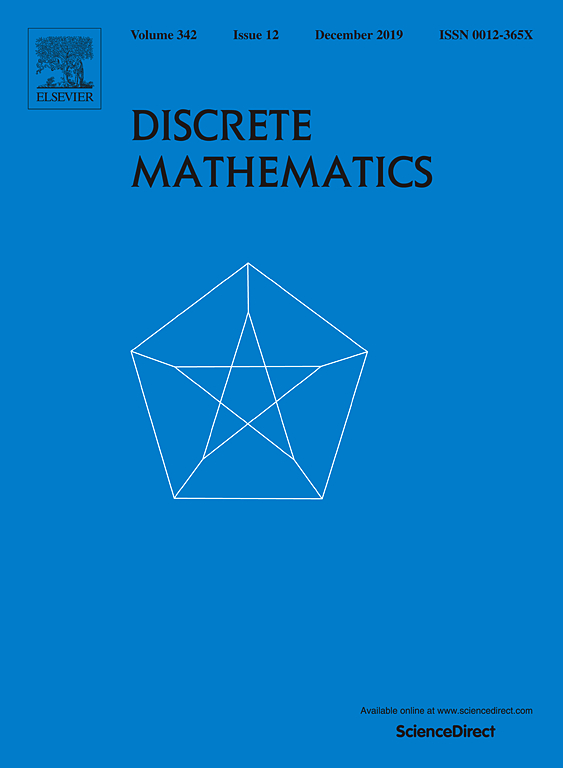
\includegraphics[width=0.3\textwidth]{figures/journal.jpg}
\end{figure}
\end{frame}

\section{Today}

\begin{frame}{Today}
\begin{table}
\def\arraystretch{1.5}
\raggedright
\begin{tabular}{r c l}
\textbf{Motivation} &-& Why this paper?\\
\textbf{Preliminaries} &-& What do you need to know?\\
\textbf{Purpose} &-& What did the authors try to find out?\\
\textbf{Theorems} &-& How did they do it?\\
\textbf{Conclusion} &-& Did you remember anything?\\
\end{tabular}
\end{table}
\end{frame}

\section{Motivation}

\begin{frame}{Why this Paper? - I}
\begin{itemize}[itemsep=0.3cm]
\item[$\blacktriangleright$] Sudoku
\item[$\blacktriangleright$] Scheduling
\item[$\blacktriangleright$] Map Colouring
\item[$\blacktriangleright$] Register allocation
\item[$\blacktriangleright$] Mobile Radio Frequency Assignment
\end{itemize}
\begin{figure}
\centering
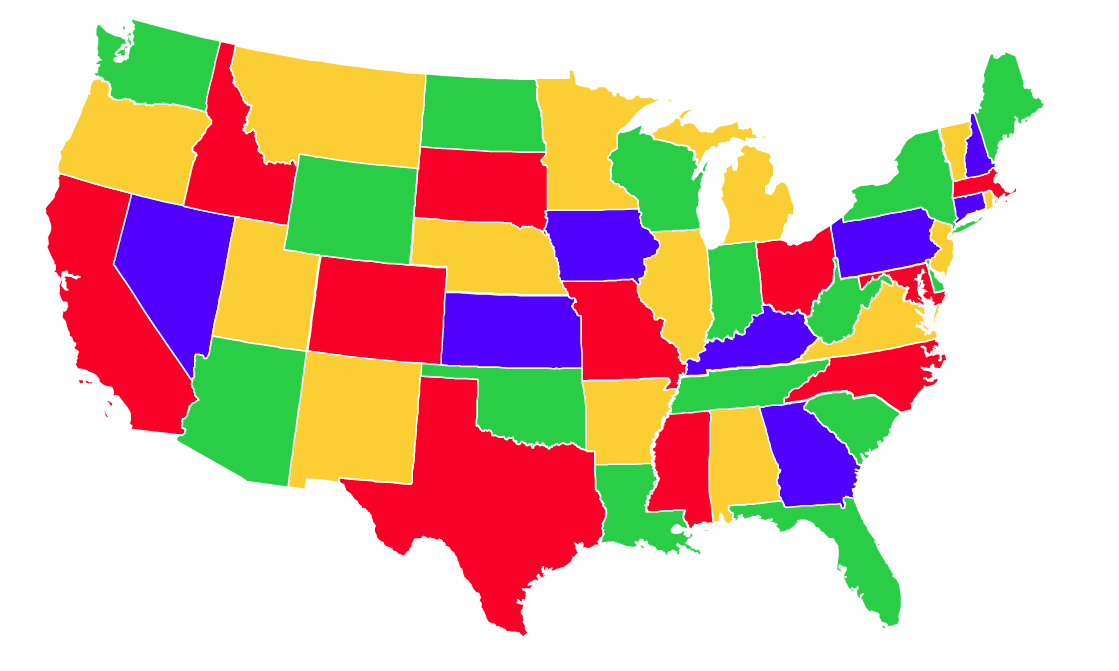
\includegraphics[width=0.5\textwidth]{figures/map2.png}
\end{figure}
\end{frame}

\begin{frame}{Why this Paper? - II}
\begin{itemize}[itemsep=0.5cm]
\item Planar graphs have been well studied.
\item Planar graph with girth at least 5 are:
\begin{itemize}[itemsep=0.5cm]
\item $(4,4)$-colourable (Skrekovski, 2000).
\item $(2,6)$-colourable (Borodin and Kostochka, 2014).
\item $(3,5)$-colourable (Choi and Raspaud, 2015).
\end{itemize}
\end{itemize}
\end{frame}

\section{Prelminaries}

\begin{frame}{Girth}
\begin{itemize}
\item[$\blacktriangleright$] The minimum length of a cycle contained in a graph $G$ is the \textbf{girth} $g(G)$ of $G$.
\end{itemize}
\begin{figure}[!tbp]
\centering
\begin{minipage}[b]{0.4\textwidth}
\includegraphics[width=\textwidth,height=3.25cm]{figures/girth.pdf}
\end{minipage}
\hfill
\begin{minipage}[b]{0.4\textwidth}
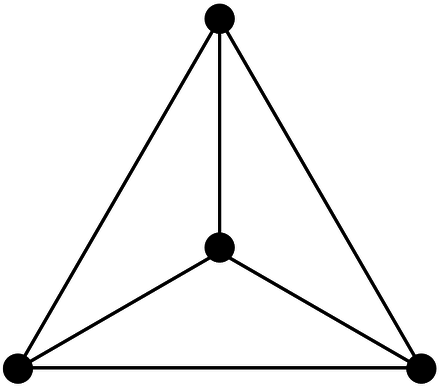
\includegraphics[width=\textwidth,height=3.25cm]{figures/triangle.png}
\end{minipage}
\caption{The Petersen graph has girth 5. The planar $K_4$ has girth 3. \cite{girth}}
\end{figure}
\end{frame}

\begin{frame}{Defective colouring - I}
\begin{itemize}
\item[$\blacktriangleright$] A $(k, d)$-colouring of $G$ is a coloring of its vertices with $k$ colours such that each vertex $v$ has at most $d$ neighbours having the same colour as the vertex $v$. 
\end{itemize}
\begin{figure}
\centering
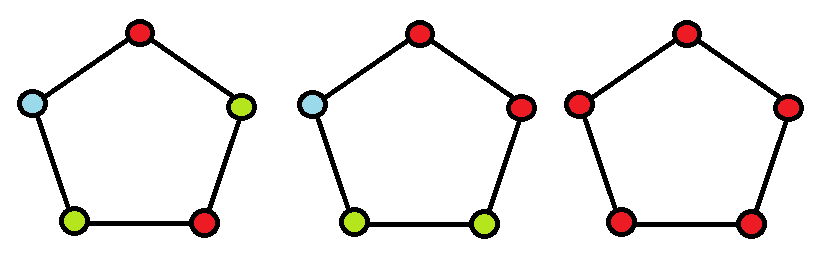
\includegraphics[width=0.8\textwidth]{figures/defect.png}
\caption{Defective colouring of a cycle on five vertices when $d = 0, 1, 2$. \cite{defect}}
\label{fig:defect}
\end{figure}
\end{frame}

\begin{frame}{Defective colouring - II}
\begin{itemize}
\item[$\blacktriangleright$] The minimum number of colours $k$ required for which $G$ is $(k, d)$-colourable is called the $d$-defective chromatic number, $\chi_d(G)$.
\end{itemize}
\begin{align*}
&\chi_{0}(C_{5})=\chi (C_{5})=3\\
&\chi_{1}(C_{5})=3\\
&\chi_{2}(C_{n})=1;\forall n\in \mathbb {N} 
\end{align*}
\begin{figure}
\centering
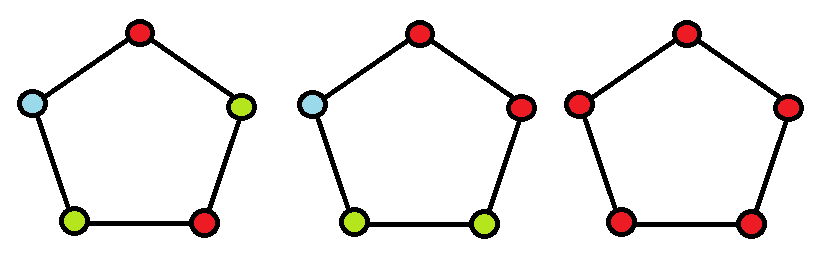
\includegraphics[width=0.6\textwidth]{figures/defect.png}
\caption{Defective colouring of a cycle on five vertices when $d = 0, 1, 2$. \cite{defect}}
\end{figure}
\end{frame}

\section{Purpose}

\begin{frame}{Purpose}
\begin{itemize}[itemsep=1cm]
\item[$\blacktriangleright$] It is known that for each pair $(k, d)$, there exists a planar graph with girth $4$ that is not $(k, d)$-colourable.
\item[$\blacktriangleright$] This sparked the interest in finding the pairs $(k, d)$ such that planar graphs with girth at least $5$ are $(k, d)$-colourable.
\end{itemize}
\end{frame}

\begin{frame}{Previous Knowledge}
\begin{itemize}
\item[$\blacktriangleright$] Improper colouring of planar graphs with girth at least 5.
\end{itemize}
\begin{theorem}[1.1]
Given $k\leq d$, planar graphs with girth $\geq5$ are $(k,d)$-colourable if
\vspace{0.25cm}
\begin{itemize}[itemsep=0.5cm]
\item\textbf{(a)}\hspace{0.25cm}$k \geq 2$ and $k+d \geq 8$ or
\item\textbf{(b)}\hspace{0.25cm}$k=1$ and $d\geq 10$.
\end{itemize}
\end{theorem}
\end{frame}

\section{Theorems}

\begin{frame}{This Paper}
\begin{itemize}
\item[$\blacktriangleright$] Improper colouring of planar graphs with girth at least 5.
\end{itemize}
\begin{theorem}[1.1]
Given $k\leq d$, planar graphs with girth $\geq5$ are $(k,d)$-colourable if
\vspace{0.25cm}
\begin{itemize}[itemsep=0.5cm]
\item\textbf{(a)}\hspace{0.25cm}$k \geq 2$ and \st{$k+d \geq 8$} or
\item\textbf{(b)}\hspace{0.25cm}$k=1$ and $d\geq 10$.
\end{itemize}
\end{theorem}
\begin{itemize}
\item[$\blacktriangleright$] Authors reveal the first pair $(k,d)$ satisfying $k + d \leq 7$.
\end{itemize}
\end{frame}

\begin{frame}{Main Theorem}
\begin{theorem}[1.2]
Planar graphs with girth at least 5 are $(3,4)$-colourable.
\end{theorem}
\begin{itemize}[itemsep=0.5cm]
\item[$\blacktriangleright$] Structural properties of a minimum counterexample to Thm. 1.2.
\item[$\blacktriangleright$] A minimum counterexample cannot exist via discharging.
\item[$\blacktriangleright$] Theorem 1.2 proved. Q.E.D.
\end{itemize}
\end{frame}

\begin{frame}{Proof Method}
\begin{lemma}[2.1]
Every edge $xy$ of $G$ has an endpoint with degree at least 5.
\end{lemma}
\begin{lemma}[2.2]
There is no 3-vertex in $G$.
\end{lemma}
$\vdots$
\begin{lemma}[2.4]
Let $C$ be a 5-face $u_1u_2u_3u_4u_5u_6$ of $G$...
\end{lemma}
$\vdots$
\begin{lemma}[2.7]
\end{lemma}
\begin{itemize}
\item[$\blacktriangleright$] Structural properties of a minimum counterexample to Thm. 1.2. 
\end{itemize}
\end{frame}

\begin{frame}{Discharging Method - I}
\begin{itemize}[itemsep=0.5cm]
\item[$\blacktriangleright$] The presence of $G$ is used to prove the colouring result.
\item[$\blacktriangleright$] A charge is assigned to each face and each vertex of the graph.
\item[$\blacktriangleright$] The charges are assigned so that they sum to a positive number. 
\item[$\blacktriangleright$] Discharging Phase 
redistributes the charge at each face/vertex to nearby faces/vertices, as required by a set of discharging rules.
\end{itemize}
\end{frame}

\begin{frame}{Discharging Method - II}
\begin{itemize}[itemsep=0.5cm]
\item[$\blacktriangleright$] Each discharging rule maintains the sum of the charges. \item[$\blacktriangleright$] The rules are designed so that after the discharging phase each face/vertex with positive charge lies in one of the desired counterexample subgraphs.
\item[$\blacktriangleright$] Since the sum of the charges is positive, some face or vertex must have a positive charge.
\item[$\blacktriangleright$] Theorem 1.2 proved. Q.E.D.
\end{itemize}
\end{frame}

\section{Conclusion}

\begin{frame}{Conclusion}
\begin{theorem}[1.2]
Planar graphs with girth at least 5 are $(3,4)$-colourable.
\end{theorem}
\begin{itemize}[itemsep=0.5cm]
\item[$\blacktriangleright$] Structural properties of a minimum counterexample to Thm. 1.2.
\item[$\blacktriangleright$] A minimum counterexample cannot exist via discharging.
\item[$\blacktriangleright$] Theorem 1.2 proved. Q.E.D.
\end{itemize}
\end{frame}

\section{END}

\plain{}{Questions?}

\begin{frame}{Acknowledgements}
\begin{table}
\centering
\begin{tabular}{l l}
Latex Beamer: & \url{github.com/matze/mtheme}\\
& \\
& \\
GitHub: & \url{github.com/GaPhil/kth-sf2740}
\end{tabular}
\end{table}
\end{frame}

\begin{frame}{Sources}
\bibliography{bibl}
\nocite{*}    
\end{frame}

\end{document}